\section{Electrical Systems}

The electrical control system for LARRE is still currently under development. The control board was developed by Micheal Conrad. The control board consists of a  Xilinx Zynq 7000 \footnote{https://www.xilinx.com/products/silicon-devices/soc/zynq-7000.html}  field-programmable gate arrays (FPGAs) as the primary controller for the exoskeleton. This allows for high speed communication with the motors and sensors. The control board is shown in \autoref{fig:controlboard}. The board as built in SPI and I2C communication for talking the external devices. This allow communication with the attached IMUs and motor controller. The large blocks are used to collected the sensor information from the sensors on the left and right leg respectively. Currently the collected data is being sent over the serial line, which can be read by a computer for validation and verification. The are six ports on the board allowing for SPI communication to external devices such as IMUs, Serial devices, and motor controllers. 


\begin{figure}
    \centering
    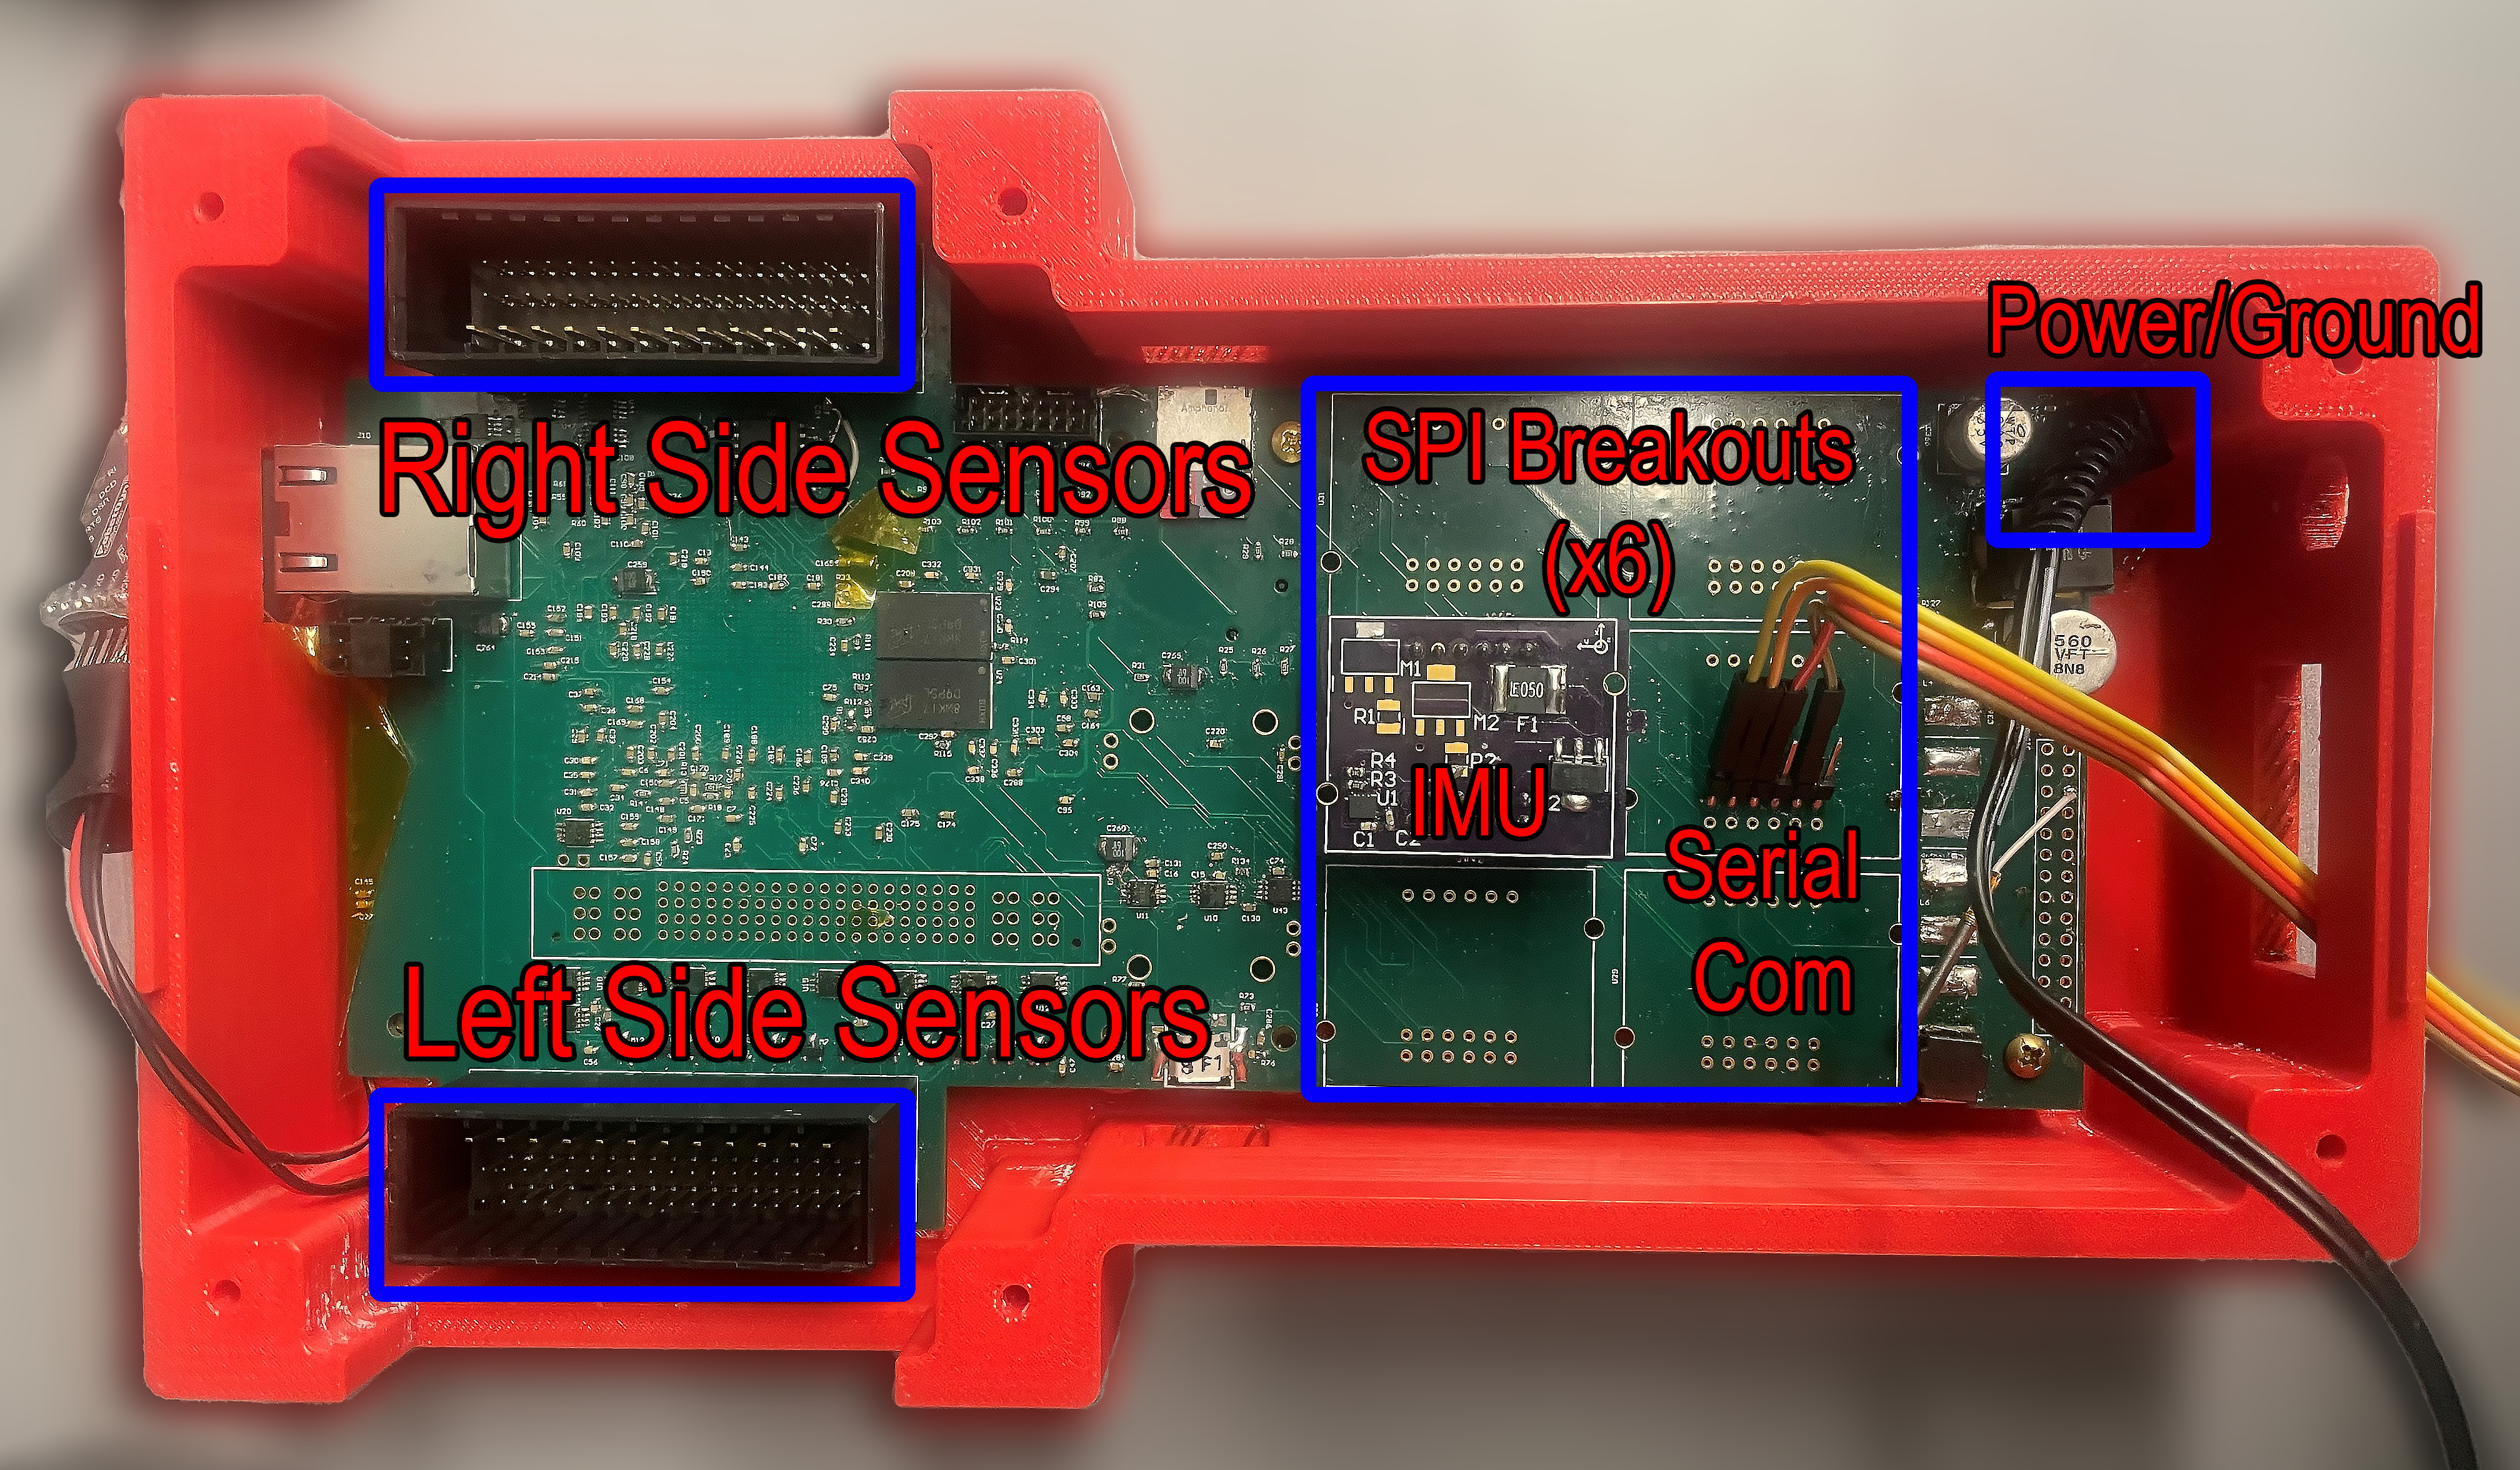
\includegraphics[width=\columnwidth]{images/mech_design/control_board_edit.png}
    \caption[LARRE Control Board]{Main LARRE Control Board with a built in FPGA for development. The board as built in SPI and I2C communication for motor control and sensors handling. The board can be programmed using a mirco SD card. }
    \label{fig:controlboard}
\end{figure}


A custom PCB with an integrated inertial measurement unit (IMU) was used to consolidate the sensor information and send it to the main collection board. The circute diagram and final board is shown in \autoref{fig:imu_circut}. The custom PCBs were placed on each of the leg segments (thigh, shank, foot) for six in total. Cables run down from the main control board the leg and snap into each of the IMU boards.  This allows for the collection of all the sensor information into a clean line. The board is powered by a 3.3V line which provides power to the IMU, pot, and FSR sensors.


\begin{figure}
    \centering
    \includegraphics[scale=0.23]{images/mech_design/IMU_diagram.png}
    \caption[Custom PCB Diagram]{Custom PCB diagram with ports for data collection and built in IMU sensor. The board collected the sensor information form the pot, IMU, and FSRs and sends it back up to the main control board.}
    \label{fig:imu_circut}
\end{figure}

A BMI160 \footnote{https://www.bosch-sensortec.com/products/motion-sensors/imus/bmi160/} (BMI160, Bosch Sensortec GmbH 2022) IMU was placed on the each of the boards with an additional IMU placed on the back of the system. This IMUs have built 3DoF gyro scope and 3DoF accelerometer sensors. This allows for the orientation and velocity of the segment to be measured. 

Each of the joints as a potentiometer that is co-axil with joint. These is used to measure the current angle of the joint. A Bourns 10K, with $300^{\circ}$ of resolution, and a D shaft was potenotmeter was used (PDF241-S425F-103B0, BOURNS inc, 1200 Columbia Ave. Riverside, CA 92507-2129, USA). As described above each of the AFOs have three built in OMITE FSRs for measuring the center of pressure of the foot. Other features of the PCM include ports for cliff sensors for detecting the edge of floor or stair case and a high power routing for a solenoid for use in the wrap spring clutch knee. 


